\documentclass[11pt,a4paper]{article}
\usepackage{fontspec}

\usepackage{xcolor}
\usepackage{tikz}
\usetikzlibrary{calc, shapes.geometric}
\usepackage{amsmath, amssymb}
\usepackage{pgfplots}
\pgfplotsset{compat=1.18}
\usepackage[most]{tcolorbox}

\definecolor{elfgreen}{RGB}{25, 89, 50}
\definecolor{elfgold}{RGB}{212, 175, 55}
\definecolor{parchment}{RGB}{245, 238, 220}

\pgfplotsset{
    colormap={elvenmagic}{
        color(0cm)=(elfgreen!20!black);
        color(1cm)=(elfgreen);
        color(2cm)=(elfgold);
        color(3cm)=(parchment)
    }
}

\begin{document}

\begin{titlepage}
    \pagecolor{parchment}
    \begin{tikzpicture}[remember picture,overlay]
        % Cadre extérieur doré
        \draw[elfgold, line width=3pt, rounded corners=15pt] 
            ($(current page.north west) + (1.5cm,-1.5cm)$) 
            rectangle 
            ($(current page.south east) + (-1.5cm,1.5cm)$);
            
        % Cadre intérieur vert
        \draw[elfgreen, line width=1pt, rounded corners=10pt] 
            ($(current page.north west) + (1.8cm,-1.8cm)$) 
            rectangle 
            ($(current page.south east) + (-1.8cm,1.8cm)$);

        % Étoiles elfiques dans les coins
        \node[star, star points=4, star point ratio=2, fill=elfgold, inner sep=3pt] 
            at ($(current page.north west) + (1.5cm,-1.5cm)$) {};
        \node[star, star points=4, star point ratio=2, fill=elfgold, inner sep=3pt] 
            at ($(current page.north east) + (-1.5cm,-1.5cm)$) {};
        \node[star, star points=4, star point ratio=2, fill=elfgold, inner sep=3pt] 
            at ($(current page.south west) + (1.5cm,1.5cm)$) {};
        \node[star, star points=4, star point ratio=2, fill=elfgold, inner sep=3pt] 
            at ($(current page.south east) + (-1.5cm,1.5cm)$) {};
            
        % Losanges verts
        \node[diamond, fill=elfgreen, inner sep=2pt] 
            at ($(current page.north) + (0,-1.5cm)$) {};
        \node[diamond, fill=elfgreen, inner sep=2pt] 
            at ($(current page.south) + (0,1.5cm)$) {};
        \node[diamond, fill=elfgreen, inner sep=2pt] 
            at ($(current page.west) + (1.5cm,0)$) {};
        \node[diamond, fill=elfgreen, inner sep=2pt] 
            at ($(current page.east) + (-1.5cm,0)$) {};
    \end{tikzpicture}
    
    \begin{center}
        \vspace*{3.5cm}
        
        {\color{elfgreen}\fontsize{42}{50}\selectfont \textsc{Le Conte de la Terre du Milieu}}\\[1.5cm]
        
        {\color{elfgold}\fontsize{22}{26}\selectfont \textit{Voyage au cœur de l'Eriador}}\\[2.5cm]
        
        
\begin{tikzpicture}
            \draw[elfgold, line width=1.5pt] (-4,0) -- (4,0);
            \node[diamond, fill=elfgreen, inner sep=4pt] at (0,0) {};
            \node[star, star points=8, star point ratio=2.5, fill=elfgold, inner sep=3pt] at (0,0) {};
        \end{tikzpicture}\\[3cm]
        
        {\color{elfgreen}\Large \textbf{Auteur :}}\\[0.2cm]
        {\color{elfgold}\LARGE \textbf{Mon Nom}}\\[3cm]
        
        \vfill
        
        {\color{elfgreen!80}\large \textit{Chroniques de Fondcombe}} \\
        {\color{elfgreen!80}\large \today}
    \end{center}
\end{titlepage}
\pagecolor{white} % Réinitialise la couleur de fond pour le reste du document

\section{Introduction}
Bonjour ! Ceci est mon tout premier document compilé localement avec \textbf{Lua\LaTeX}, \textbf{latexmk} et \textbf{Visual Studio Code}.

\section{Test mathématique}
Une petite formule pour vérifier que tout fonctionne :
\begin{equation}
    e^{i\pi} + 1 = 0
\end{equation}

\section{La Magie de \LaTeX{} : Au-delà du Texte}

Oubliez les traitements de texte traditionnels. \LaTeX{} est un moteur de composition typographique et vectoriel d'une puissance absolue, capable d'allier la rigueur scientifique à une esthétique d'une pureté stupéfiante.

\begin{tcolorbox}[
    enhanced,
    breakable,
    colback=parchment!30!white,
    colframe=elfgreen,
    title=L'Équation Fondamentale,
    fonttitle=\bfseries\Large\scshape,
    attach boxed title to top left={xshift=8mm, yshift=-3mm},
    boxed title style={colback=elfgreen, colframe=elfgold, boxrule=1pt, arc=3mm},
    drop fuzzy shadow=elfgreen!30!black,
    interior style={top color=white, bottom color=parchment!40!white}
]
La véritable force de \LaTeX{} réside dans sa capacité à composer des mathématiques d'une complexité vertigineuse avec une harmonie parfaite. Observez l'intégrale de chemin de la mécanique quantique, magnifiquement alignée :

\begin{equation}
    \mathcal{Z} = \int \mathcal{D}\phi \; \exp\left( \frac{i}{\hbar} \int d^4x \left[ \frac{1}{2}\partial_\mu\phi\partial^\mu\phi - \frac{1}{2}m^2\phi^2 - \frac{\lambda}{4!}\phi^4 \right] \right)
\end{equation}

Chaque indice, chaque intégrale, chaque parenthèse est calculé avec une précision submillimétrique selon les règles de typographie établies par Donald Knuth et les plus grandes maisons d'édition scientifiques.
\end{tcolorbox}

\vspace{1em}

Mais \LaTeX{} ne se limite pas à l'écriture. Avec \textbf{TikZ} et \textbf{pgfplots}, il se transforme en un puissant moteur de rendu graphique. Le code source de ce document génère directement, à la compilation, la surface mathématique complexe que vous voyez ci-dessous. \textit{Rien n'est une image importée, tout est calculé mathématiquement}.

\begin{center}
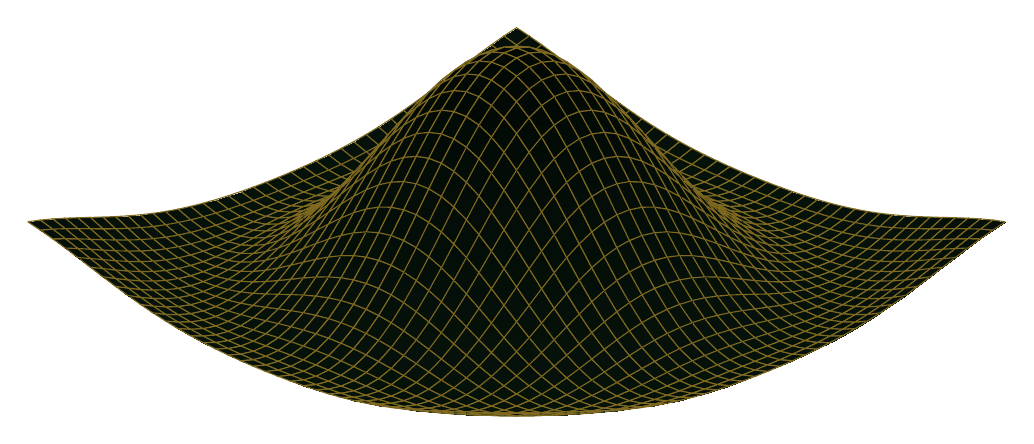
\begin{tikzpicture}
    \begin{axis}[
        hide axis,
        view={45}{45},
        width=14cm,
        height=10cm,
        colormap name=elvenmagic,
        mesh/interior colormap= {blueblack}{color=(elfgreen!20!black) color=(elfgreen!10!black)}
    ]
    \addplot3 [
        surf,
        shader=faceted interp,
        faceted color=elfgold!60!black,
        samples=40,
        domain=-5:5,
        y domain=-5:5,
        z buffer=sort
    ] {sin(deg(sqrt(x^2+y^2)))/(sqrt(x^2+y^2))};
    \end{axis}
\end{tikzpicture}
\end{center}

Observez la fluidité des dégradés (utilisant notre palette elfique sur-mesure), le calcul trigonométrique en 3 dimensions de la fonction $f(x,y) = \frac{\sin(\sqrt{x^2+y^2})}{\sqrt{x^2+y^2}}$, et le tri des polygones (z-buffer) : tout est accompli par votre compilateur ! C'est là que réside la suprématie de \LaTeX.

\end{document}